\chapter{Implementação}
Este capítulo apresenta o desenvolvimento do projeto em software, descrevendo o ambiente tecnológico utilizado para o desenvolvimento, a organização estrutural da aplicação, a implementação da Prova de Conceito (POC) de autenticação e os procedimentos iniciais de teste e integração. A ideia é demonstrar como a arquitetura do Sistema Web Administrativo da Confeitaria Bom Gosto começou a ser transformada em um programa real e funcional.

\section{Ambiente de Desenvolvimento}
O ambiente de desenvolvimento do sistema foi construído pensando na padronização e na integração contínua do código produzido pela equipe. O controle de versão é realizado através do sistema \textit{Git}, hospedado na plataforma \textit{GitHub}. Para garantir a consistência das contribuições, foram adotadas as ferramentas \textit{Husky} e \textit{Commitlint}, que operam em conjunto para forçar a padronização das mensagens de \textit{commit} segundo as regras do \textit{Conventional Commits}.

A execução do ambiente local ocorre por meio da tecnologia \textit{Docker}, permitindo que a equipe trabalhe com os mesmos pré-requisitos de infraestrutura de forma isolada. A \textit{stack} tecnológica baseia-se no \textit{framework Angular} para a construção do \textit{front-end}, ou seja, na interface, no \textit{framework Django} para o desenvolvimento da \textit{API} para o \textit{back-end} e no \textit{SGBD PostgreSQL} para o banco de dados.

\section{Estrutura da Aplicação}
A base de código foi organizada sob a abordagem de \textit{Monorepo}, centralizando todos os serviços da plataforma em um único repositório para facilitar a gestão de entregas e atividades da equipe. A estrutura de diretórios principal está dividida da seguinte forma:

\begin{figure}[H]
    \centering
    \caption{\label{fig:estrutura_repo}Estrutura do Repositório}
    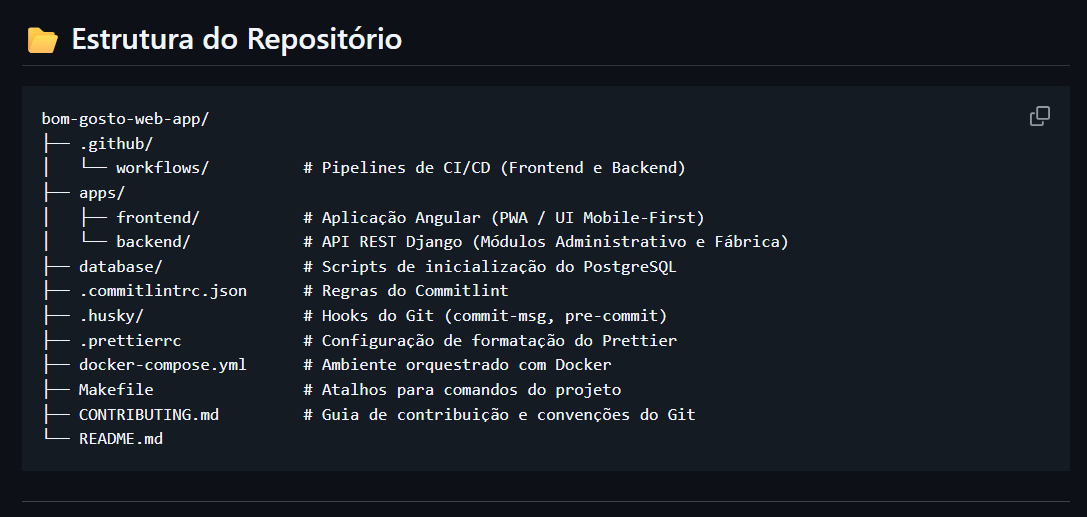
\includegraphics[width=\textwidth]{imagens/estrutura_repositorio.png}
    \legend{Fonte: Elaborado pelos autores (2026).}
\end{figure}

%%\begin{figure}[H]
%%    \centering
%%    \caption{\label{fig:diagrama_pacotes}Diagrama de Pacotes}
%%    
\includegraphics[width=\textwidth]{imagens/diagrama_pacotes.png}
%%    \legend{Fonte: Elaborado pelos autores (2026).}
%%\end{figure}

\section{Implementação dos Componentes}
Considerando o estágio atual de desenvolvimento, a equipe priorizou a validação da arquitetura por meio de uma Prova de Conceito (POC) focada no Módulo de Usuário e Segurança. Foi implementada com sucesso a funcionalidade de Autenticação no \textit{Django}, dando vida para a Regra de Negócio de Acesso Restrito (RN08).

A implementação incluiu a criação e validação dos \textit{endpoints} de segurança, como as rotas \textit{/auth/login/}, \textit{/auth/alterar-senha/}, \textit{/auth/me/} e \textit{/auth/logout/}. Além disso, o banco de dados foi estruturado física e logicamente no \textit{PostgreSQL} para manter as tabelas essenciais como o “Usuario” para a realização dessa tarefa.

\section{Integração dos Módulos}
A integração entre o \textit{front-end} e o \textit{back-end} ocorre por meio do consumo da \textit{API REST}. Em ambiente de desenvolvimento, essa comunicação é feita pelos \textit{containers Docker}, que estabelecem a rede interna necessária para que as requisições HTTP disparadas pela interface \textit{Angular} sejam processadas de maneira segura e isolada pelas rotas do \textit{Django}.

%%\begin{figure}[H]
%%    \centering
%%    \caption{\label{fig:diagrama_implantacao}Diagrama de Implantação}
%%    
\includegraphics[width=\textwidth]{imagens/diagrama_implantacao.png}
%%    \legend{Fonte: Elaborado pelos autores (2026).}
%%\end{figure}

\section{Testes Realizados}
Para garantir o funcionamento do código durante o desenvolvimento do sistema, foi estabelecido um protocolo rigoroso de testes automatizados. A cobertura de testes foi configurada utilizando o \textit{framework Pytest} para os testes unitários e de integração no \textit{back-end (API)}, enquanto o \textit{framework Jest} foi usado para avaliar o comportamento dos componentes da interface no \textit{front-end}.

\section{Resultados Obtidos}
O estágio atual do projeto mostra a aptidão de desenvolvimento do projeto. A validação da da Autenticação e a configuração bem-sucedida do \textit{monorepo} e dos testes automatizados comprovam que a infraestrutura base está pronta para receber as regras de negócio mais complexas da confeitaria.

\section{Limitações da Implementação}

Como limitação da fase presente da implementação, ressalta-se que o sistema encontra-se em etapa de estruturação de infraestrutura e segurança. Os mega-componentes focados no processamento comercial e operacional como o gerenciamento de Pedidos, a baixa de Estoque e o controle de Finanças estão definidos de maneira conceitual e comportamental, mas ainda estão em desenvolvimento da sua lógica, e aos poucos será implementado e integrado ao restante dos módulos para gerar a versão final da aplicação.

